\vspace{0.5cm}

Tomando como base la clase proporcionada por el profesor \texttt{VecR2} y se modificaron tanto los atributos, como los métodos a conveniencia para poder manejar vectores en $3$ dimensiones. Se crean los 3 archivos a utilizar \textit{t1ll3.cpp}, \textit{VecR3.cpp} y \textit{VecR3.hpp} (adjuntos a este documento). Dicho esto, se agregan los operadores $+$, $-$, $*$ (escalar y producto punto), $=$, $==$, $/$ y $\%$ (producto cruz). Cuyos métodos se pueden ver a continuación:
\begin{lstlisting}
/* Magnitud */
float VecR3::Magnitud() const
{
    return std::sqrt( Xcor*Xcor + Ycor*Ycor + Zcor*Zcor );
}


/* Operador suma */
VecR3 VecR3::operator+( const VecR3 &avec) const
{

    VecR3 tmp;

    tmp.Xcor = this->Xcor + avec.Xcor;
    tmp.Ycor = this->Ycor + avec.Ycor;
    tmp.Zcor = this->Zcor + avec.Zcor;

    return tmp;
}


/* Operador Resta */
VecR3 VecR3::operator-( const VecR3 &avec) const
{
  VecR3 tmp;

  tmp.Xcor = this->Xcor - avec.Xcor;
  tmp.Ycor = this->Ycor - avec.Ycor;
  tmp.Zcor = this->Zcor - avec.Zcor;

  return tmp;
}


/* Operador Producto punto */
float VecR3::operator*( const VecR3 &avec ) const
{
    /* Ver los comentarios de operator+ */
    float tmp;

    tmp = this->Xcor * avec.Xcor + this->Ycor * avec.Ycor + this->Zcor * avec.Zcor;

    return tmp;
}


/* Calcula el producto cruz de dos vectores */
VecR3 operator%( const VecR3 &avec )
{
  VecR3 tmp;

  tmp.Xcor = this->Ycor * avec.Zcor - this->Zcor * avec.Ycor;
  tmp.Ycor = this->Xcor * avec.Zcor - this->Zcor * avec.Xcor;
  tmp.Zcor = this->Xcor * avec.Ycor - this->Ycor * avec.Xcor;


  return tmp;
}


/* Operador de asignacion */
VecR3 VecR3::operator=( const VecR3 &avec)
{
    /* El vector que llama el operador es el que
     * esta al lado izquierdo de este, y el que
     * esta al lado derecho se pasa como argumento
     * por lo que a "this" se le debe asignar el
     * valor del argumento */
    this->Xcor = avec.Xcor;
    this->Ycor = avec.Ycor;
    this->Zcor = avec.Zcor;

    return (*this);
}


/* Operador producto por escalar */
VecR3 operator*( const float &aesc, const VecR3 &avec )
{
    VecR3 tmp;
    tmp.Xcor = aesc*avec.Xcor;
    tmp.Ycor = aesc*avec.Ycor;
    tmp.Zcor = aesc*avec.Zcor;

    return tmp;
}


/* Operador division por escalar */
VecR3 operator/( const float &aesc, const VecR3 &avec )
{
  VecR3 tmp;
  tmp.Xcor = (1/aesc)*avec.Xcor;
  tmp.Ycor = (1/aesc)*avec.Ycor;
  tmp.Zcor = (1/aesc)*avec.Zcor;

  return tmp;
}



/* Despliega un vector con cout */
std::ostream &operator<<( std::ostream &salida, const VecR3 &avec )
{
    /* Se decide el tipo de salida en funcion del valor del atributo
     * de clase Polar. */
    if( VecR3::Polar )
    {
        /* Se calcula el angulo polar del vector. La magnitud
         * se obtiene del metodo ya implementado */
        float ang = std::atan2( avec.Ycor , avec.Xcor );
        salida << "( " << avec.Magnitud() << " < " << ang << " )";
    }
    else
        salida << "( " << avec.Xcor << ", " << avec.Ycor << ", " << avec.Zcor << " )";

    return salida;
\end{lstlisting}


Con estos operadores definidos, la salida probandolos es la siguiente:
\begin{figure}[H]
	\centering
	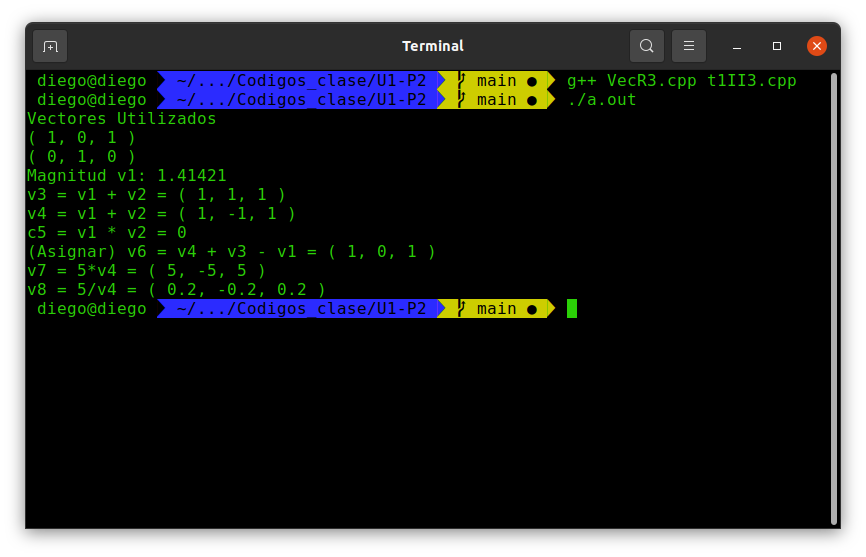
\includegraphics[scale=0.5]{./img/output.png}
	\caption{Salida del programa representando los resultados al utilizar los distintos operadores.}
	\label{output}
\end{figure}
